\section{Інтерполювання функцій}
\subsection{Постановка задачі інтерполювання}
Нехай функція $f(x) \in C([a,b])$ задана своїми значеннями $y_i = f(x_i)$, $x_i \in [a,b]$, $i = \overline{0,n}$, причому при $x_i \ne x_j$ для $i \ne j$. \\

Функція $\Phi(x)$ називається \textit{інтерполюючою} для $f(x)$ на сітці $\{x_i\}_{i=0}^n$, якщо $\Phi(x_i) = y_i$, $i = \overline{0,n}$. \\

Задача інтерполювання функції має не єдиний розв'язок. Виберемо систему лінійно незалежних функцій $\{\phi_k(x)\}_{k=0}^n$, $\phi_k(x) \in C([a,b])$ і побудуємо лінійну комбінацію \begin{equation} \label{eq:6.1} \Phi(x) = \Phi_n(x) = \Sum_{k=0}^n c_k \cdot \phi_k(x), \end{equation} яка називається \textit{узагальненим багаточленом}. Умови інтерполювання дають СЛАР \begin{equation} \label{eq:6.2} \Sum_{k=0}^n c_k \cdot \phi_k(x_i) = y_i, \quad i = \overline{1, n} \end{equation} розв'язком якої є $\vec c = (c_0, \ldots, c_n)$. Якщо \[ D(x_0, \ldots, x_n) = \begin{vmatrix} \phi_0(x_0) & \cdots & \phi_n(x_0) \\  \vdots & \ddots & \vdots \\ \phi_0(x_n) & \cdots & \phi_n(x_n) \end{vmatrix} \ne 0, \] то система (\ref{eq:6.2}) має єдиний розв'язок. \\

Система функцій $\{\phi_k (x)\}$, $k = \overline{0,n}$ називається системою Чебишова, якщо $\forall \{x_i\}_{i=0}^n$, $x_i\in[a,b]$, $D(x_0, \ldots, x_n)\ne 0$, $i=\overline{0,n}$, $\forall i \ne j$: $x_i \ne x_j$. \\

\textbf{Приклади} систем Чебишова:
\begin{enumerate}
    \item $\phi_k(x) = x^k$ -- алгебраїчна система. \\

    Визначник $D(x_0, \ldots, x_n) \ne 0$ є визначником Вандермонда: \[ D(x_0, \ldots, x_n) = \begin{vmatrix} 1 & x_0 & \cdots & x_0^n \\ \vdots & \vdots & \ddots & \vdots \\ 1 & x_n & \cdots & x_n^n \end{vmatrix} = \Prod_{0 \le k \le m \le n} (x_k - x_m) \ne 0, \]
    \item $\phi_k (x) = L_k(x)$ -- ортогональні багаточлени Лежандра; $\phi_k(x) = T_k(x)$ -- ортогональні багаточлени Чебишова.
    \item $\phi_k(x): 1, \cos(x), \sin(x), \ldots, \cos(nx), \sin(nx)$.\\

    Тоді \[\Phi_n(x) = T_n(x) = a_0 + \Sum_{k=1}^n(a_k\cdot\cos(kx) + b_k\cdot\sin(kx))\] -- тригонометричний багаточлен.
\end{enumerate}
\subsection{Інтерполяційна формула Лагранжа}
Якщо $\phi_k(x) = x^k$, то \[\Phi_n(x) = P_n(x) = \Sum_{k=0}^n c_k \cdot x^k.\] Задача інтерполювання функції $f(x)$ алгебраїчним, багаточленом полягає в знаходженні коефіцієнтів $c_k$, $k = \overline{0,n}$ для яких виконується умова $f(x_i) = \phi(x_i)$, $i = \overline{0, n}$. \\

Представимо інтерполяційний багаточлен у вигляді \begin{equation} \label{eq:6.3} P_n(x) = L_n(x) + \Sum_{k=0}^n f(x_k)\cdot\Phi_k^{(n)}(x). \end{equation} Тут $L_n(x)$ -- \textit{інтерполяційний поліном}; $\Phi_k^{(n)}(x)$ -- поліноми $n$-го степеня, які називають множниками Лагранжа. З умови $L_n(x_i)=f(x_i)$ випливає, що множник Лагранжа повинен задовольняти умови \begin{equation} \label{eq:6.4} \Phi_k^{(n)} (x_i) = \delta_{i,k}. \end{equation} Так як $\Phi_k^{(n)}(x)$ -- багаточлен степеня $n$, то він має вигляд \[ \Phi_k^{(n)}(x) = A_k\cdot(x-x_0)\cdot\ldots\cdot(x-x_{k-1})\cdot(x-x_{k+1})\cdot\ldots\cdot(x-x_n), \] де $A_k$ -- число. Знайдемо його з умови $\Phi_k^{(n)}(x_k) = 1$: \[ A_k = \dfrac{1}{(x_k-x_0)\cdot\ldots\cdot(x_k-x_{k-1})\cdot(x_k-x_{k+1})\cdot\ldots\cdot(x_k-x_n)}. \] Таким чином багаточлен $\Phi_k^{(n)}(x)$ мають вигляд: \begin{equation} \label{eq:6.5} \Phi_k^{(n)} (x) = \dfrac{(x-x_0)\cdot\ldots\cdot(x-x_{k-1})\cdot(x-x_{k+1})\cdot\ldots\cdot(x-x_n)}{(x_k-x_0)\cdot\ldots\cdot(x_k-x_{k-1})\cdot(x_k-x_{k+1})\cdot\ldots\cdot(x_k-x_n)} \end{equation} Позначивши \[\omega_n(x) = \Prod_{i=0}^n(x-x_i),\] маємо \[\Phi_k^{(n)}(x) = \dfrac{\omega_n(x)}{(x-x_k)\cdot\omega_n'(x_k)}.\] Остаточно формула Лагранжа має вигляд \begin{equation} \label{eq:6.6} L_n(x) = \Sum_{k=0}^n f(x_k)\cdot\dfrac{\omega_n(x)}{(x-x_k)\cdot\omega_n'(x_k)} \end{equation}
\subsection{Залишковий член інтерполяційного полінома}
В заданих точках (точки інтерполювання) значення функції та полінома співпадають, але в інших точках в загальному випадку не співпадають. Отже доцільно розглянути питання про похибку інтерполювання. \\

Замінюючи функцію $f(x)$ на $L_n(x)$ ми допускаємо похибку $r_n(x)=f(x)-L_n(x)$. Це \textit{залишковий член} інтерполювання. \\

З означення випливає, що, $r_n(x_i)=0$, $x_i\in[a,b]$. Оцінимо похибку у кожній точці $x\in[a,b]$. Введемо допоміжну функцію: \[g(t)=f(t)-L_n(t)-K\cdot\omega_n(t), \quad t\in[a,b], \quad g(x_i)=0, \quad i = \overline{0,n}.\] Знайдемо таке $K$, щоб $g(x)=0$, в деякій точці $x\in[a,b]$, $x\ne x_i$, $i=\overline{0,n}$. Легко бачити, що \[ K = \dfrac{f(x)-L_n(x)}{\omega_n(x)}. \] Припустимо що $f(x)\in C^{(n+1)}([a,b])$, тоді $g(t)\in C^{(n+1)}([a,b])$. Функція $g(t) = 0$ в $(n+2)$-х точках, а саме $t = x $, $t = x_i$, $i = \overline{0,n}$. З теореми Ролля випливає, що існує $(n+1)$-а точка, де $g'(t_i)=0$, $i = \overline{0,n}$. Продовжуючи цей процес, отримаємо, що існує хоча б одна $\xi \in [a,b]$ така, що $g^{(n+1)} (\xi) = 0$. Так як \[g^{(n+1)}(t) = f^{(n+1)}-0-K\cdot(n+1)!,\] то $\exists \xi$, що \[ g^{(n+1)}(\xi) = f^{(n+1)}(\xi)-(n+1)!\cdot\dfrac{f(x)-L_n(x)}{\omega_n(x)}=0.\] Звідси \begin{equation} \label{eq:6.7} r_n(x) = f(x) - L_n(x) = \dfrac{f^{(n+1)}(\xi)}{(n+1)!}\cdot\omega_n(x). \end{equation} Оскільки $\xi$ невідомо, то використовують \textit{оцінку залишкового члена}: \begin{equation} \label{eq:6.8} |r_n(x)| = |f(x) - L_n(x)| \le \dfrac{M_{n+1}}{(n+1)!}\cdot|\omega_n(x)|, \end{equation}
де $M_{n+1} = \Sup_{x\in[a,b]} |f^{(n+1)}(x)|$.
\subsection{Багаточлени Чебишова. Мінімізація залишкового члена інтерполяційного полінома}
Як вибрати вузли інтерполяції щоб похибка інтерполювання була мінімальною? Спочатку обґрунтуємо теоретичний апарат, завдяки якому будемо досліджувати це питання. \\

\textit{Багаточленом Чебишова ($n$-того степеня, 1–го роду)} називається поліном, який задається такими рекурентними співвідношеннями \begin{equation} \label{eq:6.9} T_{n+1}(x)-2x\cdot T_n(x)+T_{n-1}(x) = 0, \end{equation} \begin{equation} \label{eq:6.10} T_0(x) = 1, \quad T_1(x) = x. \end{equation} Знайдемо явний вигляд багаточлена Чебишова. Будемо шукати розв'язок рівняння (\ref{eq:6.9}) у вигляді $T_n(x) = q^n$, де $q = q(x)$. Підставивши в (\ref{eq:6.9}), отримуємо характеристичне рівняння $q^2 - 2xq + 1 = 0$. Тоді при $|x|\ge1\Rightarrow q_{1,2}=x\pm\sqrt{x^2-1}$, а при $|x|<1\Rightarrow q_{1,2}=\cos(\phi)\pm i\sin(\phi)$, $\phi = \arccos(x)$. \\

Розглянемо обидва випадки детальніше: 
\begin{enumerate}
    \item при $|x| \le 1$: $T_n(x) = A\cdot\cos(n\phi) + B\cdot\sin(n\phi)$. З (\ref{eq:6.10}) випливає $A=1$, $B=0$ і тому \begin{equation} \label{eq:6.11} T_n(x) = \cos(n \arccos (x)). \end{equation}
    \item при $|x| > 1$: \begin{equation} \label{eq:6.12} T_n(x) = \dfrac12 \left(\left(x+\sqrt{x^2-1}\right)^n+\left(x-\sqrt{x^2-1}\right)^n\right). \end{equation}
\end{enumerate}
Знайдемо нулі та екстремуми багаточлена Чебишова: $T_n(x) = 0$, $x\in[-1,1]$, $\cos(n \arccos(x)) = 0$, $\arccos(x) = \frac{2k+1}{2n}\pi$, $k=\overline{0,n-1}$. \\

Отже \textit{нулі багаточлена Чебишова}: \[ x_k = \cos \left( \dfrac{(2k+1)\pi}{2n} \right) \in [-1,1], \quad k=\overline{0,n-1}. \] \textit{Локальні екстремуми багаточлена Чебишова} на $x\in[-1,1]$: \[ x_k' = \cos \left( \dfrac{k\pi}{2n} \right), \quad k=\overline{0,n}.\] Коефіцієнт при старшому члені багаточлена дорівнює $2^{n-1}$. Введемо \textit{нормований багаточлен Чебишова} $\overline{T}_n(x) = 2^{1-n} T_n(x) = x^n + \ldots$ Тоді \[ \left\|\overline{T}_n\right\|_{C([-1,1])} = \Max_{x\in[-1,1]} |T_n(x)| = 2^{1-n}. \] Відхиленням двох функцій $f(x)$ та $\Phi(x)$ називається величина  \[ \Delta (f, \Phi) = \| f(x) - \Phi(x)\|_{C([a,b])}. \]
\begin{theorem}[Чебишова]
    Серед усіх багаточленів $n$-го степеня з коефіцієнтом 1 при старшому степені $\overline{T}_n(x)$ найменше відхиляється від 0 на $[-1,1]$, тобто \[ \left\|\overline{T}_n(x) - 0\right\|_{C([-1,1])} = \Inf_{\overline{P}_n(x)} \left\|\overline{P}_n(x)\right\|_{C([-1,1])} = 2^{1-n}. \]
\end{theorem}
\begin{proof}
    Будемо доводити від супротивного: припустимо, що існує багаточлен, такий, що \[ \overline{Q}_n(x) < 2^{1-n}.\] Тоді $Q_{n-1}(x) = \overline{T}_n(x) - \overline{Q}_n(x)$ -- поліном степеня не вище $n-1$ і не рівний тотожньо нулю. Дослідимо його знаки: \[ \signum\left(Q_{n-1}(x_k')\right)=\signum\left(\overline{T}_n(x_k')-\overline{Q}_n(x_k')\right)=\signum\left(\overline{T}_n(x_k')\right) = \alpha\cdot(-1)^k, \quad \alpha = \pm 1. \] Значить $\exists z_k$, $k=\overline{0,n-1}$ таке, що $Q_{n-1}(z_k)=0$. Це протиріччя, бо $Q_{n-1}(x)$ -- поліном степеня $\le n - 1$.
\end{proof}
Тепер узагальнимо наш багаточлен Чебишова на довільний проміжок. Нагадаємо $T_n(t) = \cos(n \arccos t)$, $-1 \le t \le 1$. Від змінної $t \in [-1, 1]$ перейдемо до $x \in [a,b]$. Запровадимо заміну \[t = \frac{2}{b-a}x - \frac{b+a}{b-a}, \quad x=\frac{b+a}{2}+\frac{b-a}t.\] Тоді \[ T_n^{[a,b]}(t)=\overline{T}_n\left(\dfrac{2}{b-a}x-\dfrac{b+a}{b-a}\right)=2^{1-n}\cos\left(n\arccos\left(\dfrac{2x-(b+a)}{b-a}\right)\right).\] Побудований нами багаточлен Чебишова на $[a,b]$ не є нормованим. \textit{Нормований багаточлен Чебишова} на $[a,b]$: \[ \overline{T}_n^{[a,b]}(x) = \dfrac{(b-a)^n}{2^{2n-1}}\cos\left(n\arccos\left(\dfrac{2x-(b+a)}{b-a}\right)\right). \] Відповідно його нулі \[x_k = \dfrac{a+b}{2} - \dfrac{b-a}{2}t_k, \quad t_k = \cos\left(\frac{(2k+1)\pi}{2n}\right), \quad k=\overline{0,n-1},\] а точки екстремуму \[ x_k' = \dfrac{a+b}{2} - \dfrac{b-a}{2}t_k', \quad t_k' = \cos\left(\frac{k\pi}{n}\right), \quad k=\overline{0,n}.\] Теорема Чебишова вірна і у випадку $[a,b]$. Тепер $\left\|\overline{T}_n^{[a,b]}\right\|_{C([a,b])} = \frac{(b-a)^n}{2^{2n-1}}$. \\

Перейдемо до питання мінімізації залишкового члена. Нагадаємо, що \begin{equation} \label{eq:6.13} |r_n(x)| = |f(x) - L_n(x)| \le \dfrac{M_{n+1}}{(n+1)!}\cdot|\omega_n(x)|, \end{equation} де $M_{n+1} = \Max_{x\in[a,b]} |f^{(n+1)}(x)|$, $\omega_n(x)=\Prod_{i=0}^n (x-x_i)=x^{n+1} + \ldots$\\

Поставимо задачу \[ \Inf_{\overline{P}_n(x)} \Max_{x\in[a,b]} |\omega_n(x)|. \] З теоремою Чебишова $\omega_n(x) = \overline{T}_{n+1}^{[a,b]}(x)$ поліном Чебишова. Якщо співпадають поліноми, то співпадають їх нулі. Отже: $x_k$ -- вузли інтерполяції співпадають з нулями багаточлена Чебишова \[x_k = \dfrac{a+b}{2} - \dfrac{b-a}{2}t_k,\quad t_k = \cos\left(\frac{(2k+1)\pi}{2(n+1)}\right),\quad k=\overline{0,n}.\] В цьому випадку \begin{equation} \label{eq:6.14} |r_n(x)| = |f(x)-L_n(x)| \le \dfrac{M_{n+1}}{(n+1)!} \cdot \dfrac{(b-a)^{n+1}}{2^{2n+1}}. \end{equation} Цю оцінку не можна покращити! Так для $f(x) = \overline{P}_{n+1}(x) = x^{n+1} + \ldots $ її $(n+1)$ похідна дорівнює $(n+1)!$, тому $M_{n+1} = (n+1)!$. Різниця $f(x) - L_n(x) = \overline{T}_{n+1}^{[a,b]}(x)$, отже \[\Max_{x\in[a,b]} |f(x) - L_n(x)| = \dfrac{(b-a)^{n+1}}{2^{2n+1}}.\]
\subsection{Розділені різниці}
Розділені різниці є аналогом похідної для функції, що задана таблицею. \\

\textit{Розділеною різницею 1-го порядку} для функції $f(x)$ називатимемо \[ f(x_i; x_j) = \dfrac{f(x_i)-f(x_j)}{x_i-x_j}. \] \textit{Розділеною різницею 2-го порядку} для функції $f(x)$ називатимемо \[ f(x_i; x_j; x_k) = \dfrac{f(x_i;x_j)-f(x_j;x_k)}{x_i-x_k}. \] Аналогічно визначаються розділені різниці довільного порядку. \\

Наведемо деякі властивості розділених різниць:
\begin{enumerate}
    \item \[f(x_0; \ldots; x_n) = \Sum_{i=0}^n \dfrac{f(x_j)}{\Prod_{i\ne j}(x_i-x_j)}.\]
    \item Розділена різниця -- лінійний функційонал: \[ (\alpha_1 f_1 + \alpha_2 f_2)(x_0; x_1) = \alpha_1 f_1(x_0;x_1) + \alpha_2 f_2(x_0;x_1). \]
    \item Розділена різниця -- симетричний функціонал: \[ f(x_1; \ldots; x_i; \ldots; x_j; \ldots; x_n) = f(x_1; \ldots; x_j; \ldots; x_i; \ldots; x_n). \]
    \item Для $f(x) \in C^{(n)}([a,b])$ $\exists \xi \in [a,b]$: $f(x_0; x_1; \ldots; x_n) = \frac{f^{(n)}(\xi)}{n!}$.
\end{enumerate}
\begin{problem}
    Довести першу властивість розділених різниць.
\end{problem}
Таблиця розділених різниць має вигляд:
\begin{table}[H]
    \centering
    \begin{tabular}{c|ccccc}
        $x_i$ & $f_i$ & р.р.1 & р.р.2 & $\ldots$ & р.р.$n$ \\ \hline
        $x_0$ & $f(x_0)$ & & & & \\
        & & $f(x_0;x_1)$ & & & \\
        $x_1$ & $f(x_1)$ & & $f(x_0;x_1;x_2)$ & & \\
        & & $f(x_1;x_2)$ & & & \\
        $x_2$ & $f(x_2)$ & & & & \\
        $\vdots$ & $\vdots$ & $\vdots$ & $\vdots$ & $\vdots$ & \\
        $\cdots$ & $\cdots$ & $\cdots$ & $\cdots$ & $\cdots$ & $f(x_0;\ldots;x_n)$ \\
        $\vdots$ & $\vdots$ & $\vdots$ & $\vdots$ & $\vdots$ & \\
        $x_n$ & $f(x_n)$ & & & & \\
    \end{tabular}
\end{table}
\subsection{Інтерполяційна формула Ньютона}
Запишемо формулу Лагранжа інтерполяційного багаточлена
\begin{equation}
    \label{eq:6.15}
    L_n(x) = \Sum_{i=0}^n f(x_i) \cdot \dfrac{\omega_n(x)}{(x-x_i)\cdot \omega_n'(x_i)},
\end{equation}
де $\omega_n(x) = \Prod_{j=0}^n (x-x_j)$. \\

Позначимо $\Phi_j(x) = L_j(x) - L_{j-1}(x)$. Тоді, оскільки
\[ L_n(x) = L_0(x) + (L_1(x) - L_0(x)) + \ldots + (L_n(x) - L_{n-1}(x)), \]
\[ L_j(x_i) = L_{j-1}(x_i) = f(x_i), \quad i = \overline{0,j-1},\]
то
\begin{equation}
    \label{eq:6.16}
    \Phi_j(x_i) = A_j \cdot (x - x_0) \cdot \ldots \cdot (x - x_{j-1}),
\end{equation}
де $A_j$ визначається з умови $\Phi_j(x_j) = L_j(x_j) - L_{j-1}(x_j) = f(x_j) - L_{j-1}(x_j)$. Звідси
\[ \Phi_j(x) = \dfrac{f(x_j)-L_{j-1}(x_j)}{(x_j-x_0)\cdot\ldots\cdots(x_j-x_{j-1})}\cdot(x-x_0)\cdot\ldots\cdot(x-x_j).\] 
Тоді
\begin{multline*}
    A_j = \dfrac{f(x_j)-L_{j-1}(x_j)}{(x_j-x_0)\cdot\ldots\cdots(x_j-x_{j-1})} = \dfrac{f(x_j)}{(x_j-x_0)\cdot\ldots\cdots(x_j-x_{j-1})} - \\
    - \Sum_{i=0}^{j-1} \dfrac{f(x_i)}{(x_i-x_0)\cdot\ldots\cdot(x_i-x_{i-1})\cdot(x_i-x_{i+1})\cdot\ldots\cdot(x_i-x_{j-1})\cdot(x_j-x_i)} = \\
    = \dfrac{f(x_j)}{(x_j-x_0)\cdot\ldots\cdots(x_j-x_{j-1})} + \Sum_{i=0}^{j-1} \dfrac{f(x_i)}{(x_i-x_0)\cdot\ldots\cdot(x_i-x_j)} =  \\
    = \Sum_{i=0}^j \dfrac{f(x_i)}{(x_i-x_0)\cdot\ldots\cdot(x_i-x_{i-1})\cdot(x_i-x_{i+1})\cdot\ldots\cdot(x_i-x_j)} = f(x_0;\ldots;x_j).
\end{multline*}
Звідси маємо інтерполяційну формулу Ньютона вперед ($x_0 \to x_n$):
\begin{equation}
    \label{eq:6.17}
    L_n(x) = f(x_0) + f(x_0;x_1) \cdot (x-x_0) + \ldots + f(x_0;\ldots;x_n) \cdot (x-x_0) \cdot \ldots \cdot (x-x_{n-1}).
\end{equation}
Аналогічно, інтерполяційна формула Ньютона назад ($x_n\to x_0$):
\begin{multline}
    \label{eq:6.18}
    L_n(x) = f(x_n) + f(x_n;x_{n-1}) \cdot (x-x_n) + \ldots \\
    \ldots + f(x_n;\ldots;x_0) \cdot (x-x_n) \cdot \ldots \cdot (x-x_1).
\end{multline}
Маємо рекурсію за степенем багаточлена 
\[ L_n(x) = L_{n-1}(x) + f(x_0;\ldots;x_n)\cdot(x-x_0)\cdot\ldots(x-x_1).\]
Звідси \[L_n(x) = f(x_0) + (x-x_0)\cdot(f(x_0;x_1)+(x-x_1)\cdot(\cdots+(x-x_{n-1})\cdot f(x_0;x_1;\ldots;x_n)))\] і цю формулу розкриваємо починаючи з середини (це аналог схеми Горнера обчислення значення багаточлена). \\

Введемо нову формулу для похибки інтерполювання. Для $x \ne x_i$, $i = \overline{0,n}$ розглянемо розділену різницю
\[ f(x;x_0;\ldots;x_n) = \dfrac{f(x)}{(x-x_0)\cdot\ldots\cdot(x-x_n)} + \Sum_{k=0}^n \dfrac{f(x_k)}{\Prod_{i\ne k}(x-x_i)}.\]
Звідси
\begin{multline*}
    f(x) = f(x_0) \cdot \dfrac{(x-x_1)\cdot\ldots\cdot(x-x_n)}{(x_0-x_1)\cdot\ldots\cdot(x_0-x_n)} + \ldots + f(x_n) \cdot \dfrac{(x-x_1)\cdot\ldots\cdot(x-x_n)}{(x_n-x_1)\cdot\ldots\cdot(x_n-x_{n-1})} + \\
    + f(x;x_0;\ldots;x_n)\cdot(x-x_0)\cdot\ldots\cdot(x-x_n)=L_n(x)+f(x;x_0;\ldots;x_n)\cdot\omega_n(x).
\end{multline*}
Тоді похибка має вигляд
\begin{equation}
    \label{eq:6.19}
    r_n(x) = f(x) - L_n(x) = f(x;x_0;\ldots;x_n)\cdot\omega_n(x).
\end{equation}
Це нова форма для залишкового члена.\\

Порівнюючи з формулою залишкового члена в пункті (6.3), маємо
\[ f(x;x_0;\ldots;x_n) = \dfrac{f^{(n+1)}(\xi)}{(n+1)!},\]
що доводить останню властивість розділених різниць. \\

Нехай маємо сітку рівновіддалених вузлів: $x_i = a + i h$, $h = \frac{b-a}{n}$, $i = \overline{0, n}$, $x_0 = a$, $x_n = b$. Розначимо $\Delta f_0 = f_1 - f_0$, $\Delta^2f_0 = \Delta f_1 - \Delta f_0 = f_2 - 2 f_1 + f_0$, $\ldots$ -- скінченні різниці. Запишемо формули Ньютона у нових позначеннях:
\[ L_n(x) = L_n(x_0 + t h) = f_0 + t \Delta f_0 + \ldots + \dfrac{t\cdot(t-1)\cdot(t-n+1)}{n!}\cdot \Delta^n f_0, \quad t = \dfrac{x-x_0}{h}.\]
Це інтерполяційна формула Ньютона вперед по рівновіддалених вузлах.
\begin{problem}
    Побудувати інтерполяційну формулу Ньютона назад по рівновіддалених вузлах.
\end{problem}
\subsection{Інтерполювання з кратними вузлами}
Нехай $f(x)$ задана таблицею значень $f^{(j)}(x_i)$, $i=\overline{0,n}$, $j=\overline{0,k_i-1}$, $k_i$ -- кратності відповідних вузлів. Побудуємо $H_m^{(i)}(x_j) = f^{(i)}(x_j)$ -- інтерполяційний багаточлен Ерміта по кратним вузлах, де $m = \Sum_{i=1}^n k_i - 1$. \\

Якщо $k_i=1$, то $H_m(x) = L_n(x)$. \\

Для побудови $H_m(x)$ в загальному випадку для кожної точки $x_i$ введемо $k_i$ точок $x_{i,j}^\epsilon = x_i + j\epsilon$, $i=\overline{0,n}$, $j=\overline{0,k_i-1}$. З умови $\forall i$: $x_{i,k_i-1}^\epsilon = x_i + \epsilon(k-1) < x_{i+1}$ можна вибрати $\epsilon$. \\

Нехай $f(x) \in C^{(m)}([a,b])$. Запишемо інтерполяційну формулу Ньютона:
\begin{multline*} 
    L_m^\epsilon = f\left(x_{0,0}^\epsilon\right)+f\left(x_{0,0}^\epsilon;x_{0,1}^\epsilon\right)\cdot\left(x-x_{0,0}^\epsilon\right) + \ldots \\

    \ldots + f\left(x_{0,0}^\epsilon;\ldots;x_{n,k_n-1}^\epsilon\right)\cdot\left(x-x_{0,0}^\epsilon\right)\cdot\ldots\cdot\left(x-x_{n,k_n-1}^\epsilon\right).
\end{multline*}
При $\epsilon \to 0$ маємо $x_{i,j}^\epsilon \to x_i$. Крім того
\[f\left(x_{i,0}^\epsilon;\ldots;x_{i,k_i-1}^\epsilon\right)=f(x_i;\ldots;x_i)=\dfrac{f^{(k_i)}(x_i)}{k_i!}.\]
Тому $L_m^\epsilon(x)\to H_m(x)$ та
\[ R_m(x) = f(x) - H_m(x) = \dfrac{f^{(m+1)}(\xi)}{(m+1)!}\cdot \Omega_m(x),\]
де $\Omega_m(x) = (x-x_0)^{k_0}\cdot\ldots\cdot(x-x_n)^{k_n}$.
\subsection{Збіжність процесу інтерполювання}
Виникає питання, чи буде прямувати до нуля похибка інтерполювання $f(x) - L_n(x)$, якщо число вузлів $n$ збільшувати? \\

Введемо норму $\|f(x)-L_n\|_{C([a,b])} = \Max_{x\in[a,b]}|f(x)-L_n(x)|$. Тоді для довільної $f(x)\in C^{(n+1)}([a,b])$ справджується оцінка
\begin{equation}
    \label{eq:6.20}
    \| f(x) - L_n(x)\|_{C([a,b])} \le \dfrac{M_{n+1}}{(n+1)!}\|\omega_n(x)\|_{C([a,b])},
\end{equation}
де $M_{n+1} = \Max_{x\in[a,b]} |f^{(n+1)}(x)|$, $\omega_n(x) = \Prod_{i=0}^n (x-x_i)$. А яка оцінка буде для довільної неперервної функції? \\

Кажуть, що інтерполяційний процес для функції $f(x)$ \textit{збігається} в точці $x\in[a,b]$, якщо 
\[ \Lim_{n\to\infty} L_n(x) = f(x), \quad \forall \{x_i\}_{i=1}^n: h = \Max_{i=\overline{1,n}} h_i \to 0, \quad h_i = x_i - x_{i-1}.\]
Якщо $\|f(x)-L_n(x)\|_{C([a,b])} \xrightarrow[n\to\infty]{}0$, то інтерполяційний процес збігається рівномірно. \\

Розглянемо приклади поведінки інтерполяційних багаточленів при $n\to\infty$ для деяких функцій. \\

\textbf{Приклад 1}. Послідовність інтерполяційних багаточленів (сітка рівномірна), побудованих для неперервної функції $f (x) = |x|$, $-1\le x\le1$ (функція неперервна, але негладка), не збігається на $x \in [-1,1]$, крім точок $x=-1,0,1$. \\

На рисунку дано графіки самої функції (штрихова лінія) та інтерполяційного багаточлена (суцільна лінія) на рівномірній сітці $x_i = -1 + i h$, $h = \frac2n$, $i=\overline{0,n}$ для $n = 10$:
\begin{figure}[H]
    \centering
    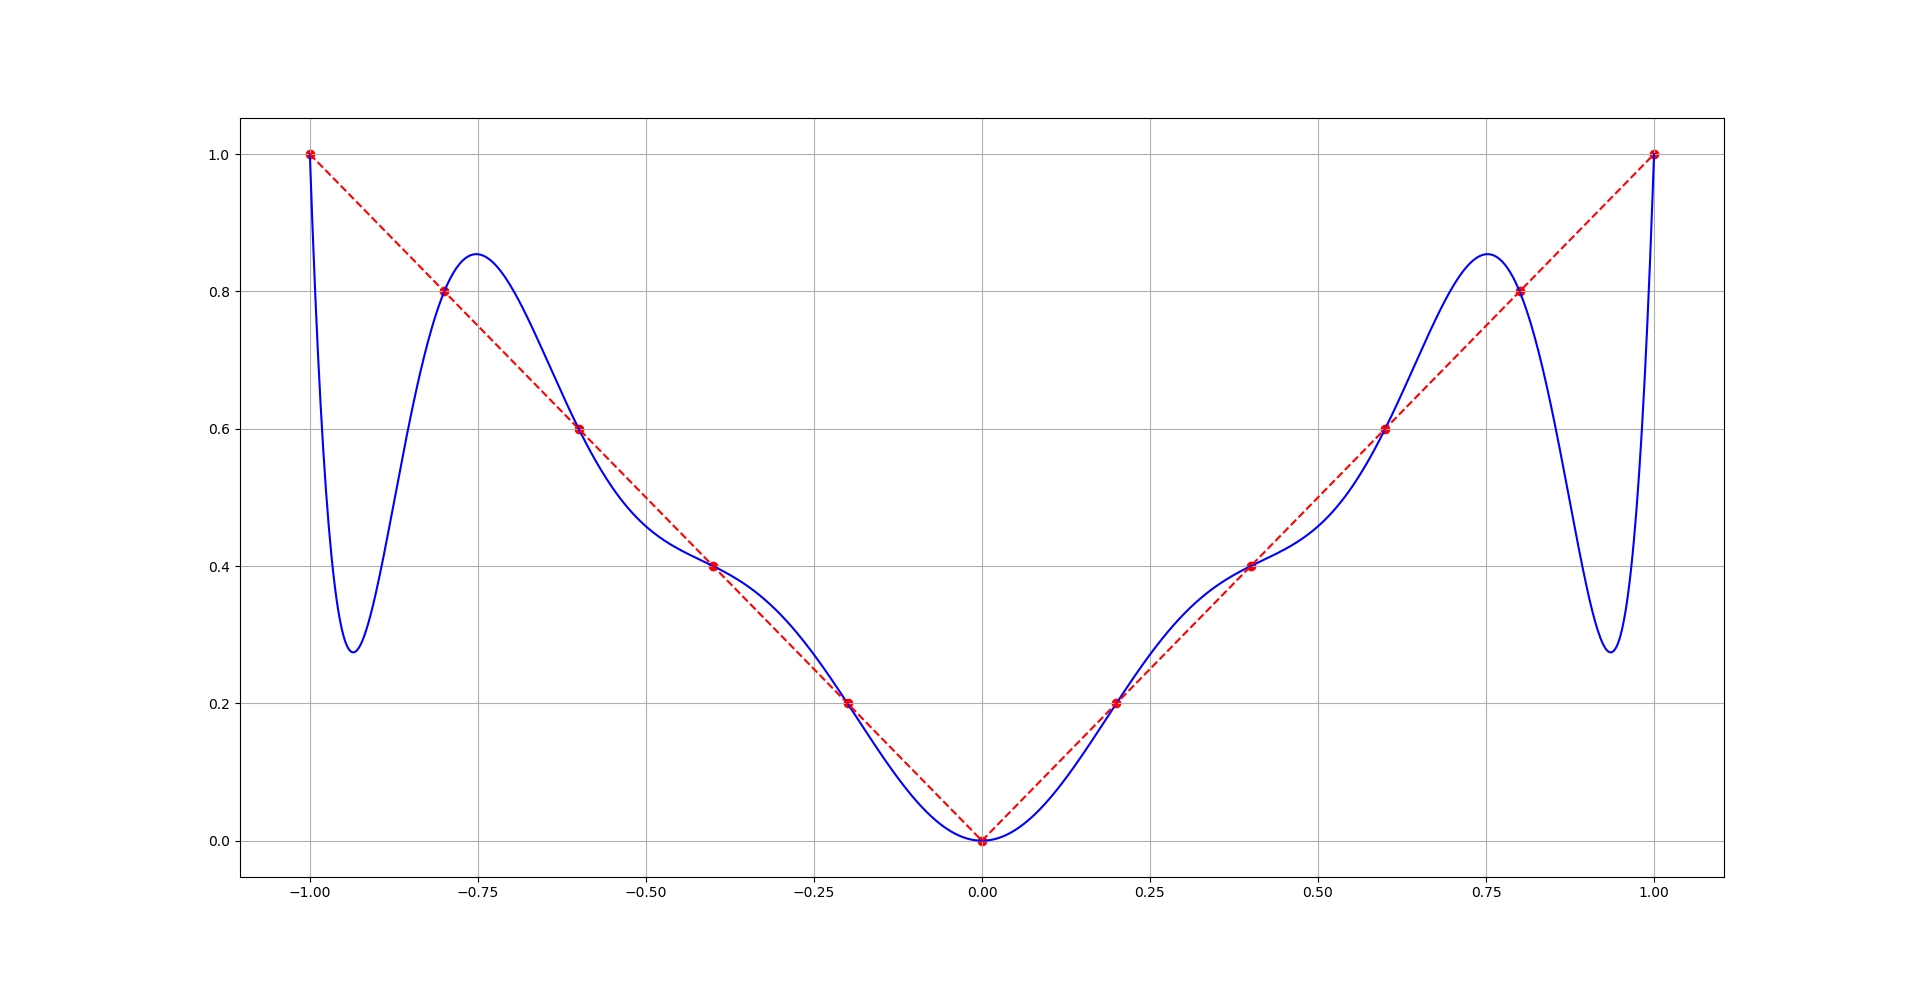
\includegraphics[width=\linewidth]{mal-4.png}
\end{figure}
\textbf{Приклад 2}. Функція Рунге $f(x) = \frac{1}{1+40x^2}$, $-1\le x\le1$ (функція аналітична!). Для рівномірної сітки $x_i = -1 + i h$, $h = \frac2n$, $i=\overline{0,n}$ маємо графіки: суцільна лінія -- інтерполяційного багаточлена; пунктирна -- самої функції для $n = 10$:
\begin{figure}[H]
    \centering
    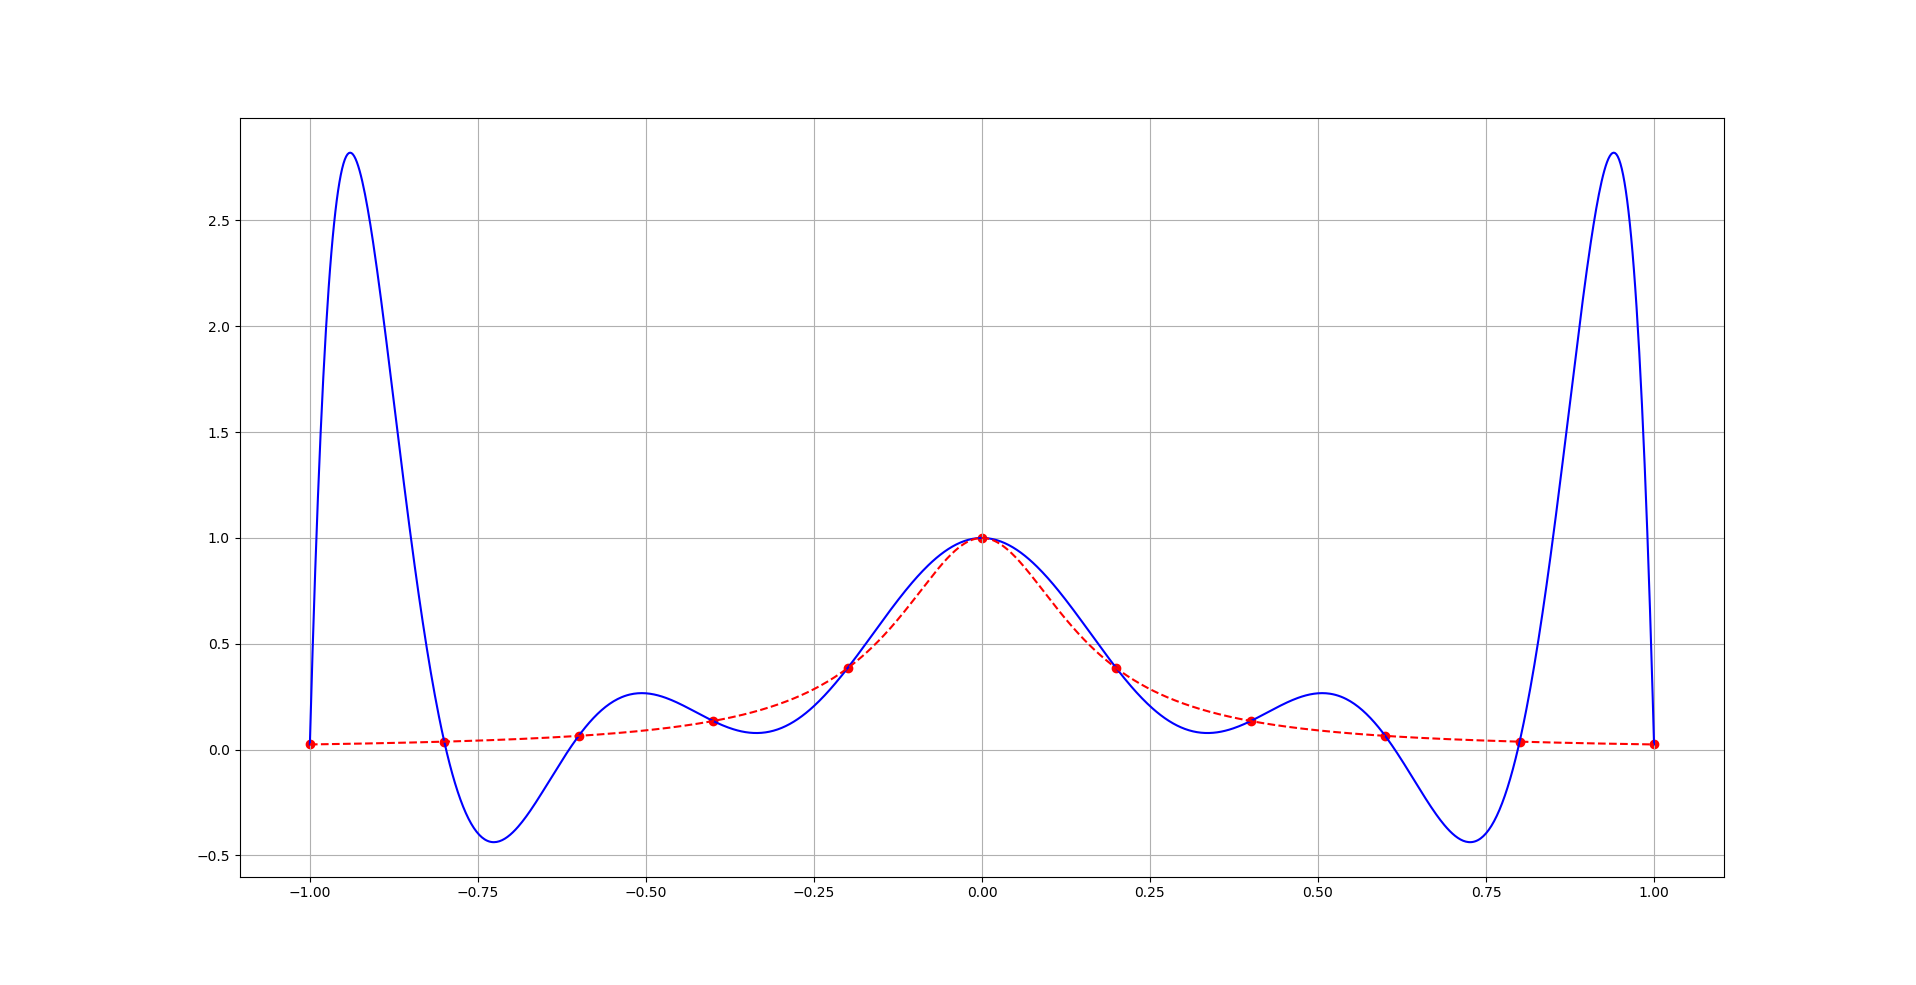
\includegraphics[width=\linewidth]{mal-5.png}
\end{figure}
Пояснити чому рівномірна сітка дає великі похибки інтерполювання біля кінців інтервалу інтерполювання допомагає наступний рисунок. На цьому рисунку суцільною лінією представлено графік функції $\omega_n = \Prod_{i=0}^n (x-x_i)$ ($n=8$) для рівномірної сітки. Як бачимо максимальні за модулем значення цієї функції припадають на кінці інтервалу.
\begin{figure}[H]
    \centering
    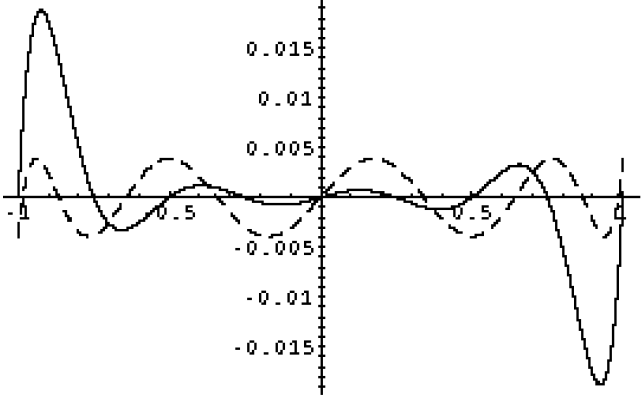
\includegraphics[width=.5\linewidth]{mal-6.png}
\end{figure}
Для порівняння на цьому ж рисунку (штрихова лінія) побудовано графік $\omega_n = \Prod_{i=0}^n (x-x_i)$, що відповідає чебишовським вузлам, які мінімізують похибку інтерполювання. Тепер відхилення $\omega_n(x)$ розподілено рівномірно по всьому проміжку інтерполювання.
\begin{theorem}[Фабера]
    $\forall \{x_i\}_{i=0}^n$ існує $f(x)\in C([a,b])$, для якої інтерполяційний процес не збігається рівномірно.
\end{theorem}
\begin{theorem}[Марцинкевича]
    $\forall f(x) \in C([a,b])$ існуюють $\{x_i\}_{i=0}^n$ такі, що послідовність $\{L_n(x)\}$ збігається рівномірно до $f(x)$.
\end{theorem}
\begin{theorem}
    Стала Лебега $\|P_n\| = \Max_{j} \Sum_{j=0}^n |\phi_j^{(n)}(x)|$, де $\phi_j^{(n)}(x) = \frac{\omega_n(x)}{(x-x_j)\cdot\omega_n'(x_i)}$.
\end{theorem}
\begin{theorem}
    Для $f(x)\in C([a,b])$:
    \[\|f(x)-L_n(x)\|_{C([a,b])} \le (1 + \|P_n\|) \cdot E_n(f),\]
    де $E_n(f) = \Inf{Q_n(x)} \|f(x)-Q_n(x)\|_{C([a,b])}$ -- відхилення багаточлена $n$-го степеня найкращого рівномірного наближення від $f(x)$.
\end{theorem}
\begin{theorem}
    Нехай $P_n^E$ -- оператор інтерполяції на рівномірній сітці, $P_n^T$ -- оператор інтерполяції на чебишовській сітці. Тоді на $[-1,1]$ маємо наближені оцінки:
    \[ \|P_n^E\|\approx C_1 \cdot 2^n, \quad \|P_n^T\|\approx C_2\cdot \ln(n).\]
\end{theorem}
Останні оцінки поясняють розбіжність процесу інтерполювання при великих $n$.
\subsection{Кусково-лінійна інтерполяція}
Інтерполяція багаточленом Лагранжа або Ньютона на відрізку $[a,b]$ з використанням великої кількості вузлів інтерполяції часто приводить до поганого наближення через розбіжність процесу інтерполювання. Для того щоб уникнути великої похибки, весь відрізок $[a,b]$ розбивають на частинні відрізки $[x_{i-1}, x_i]$ і на кожному з частинних відрізків замінюють функцію $f(x)$багаточленом невисокого степеню. В цьому і полягає кусково-поліноміальна інтерполяція. \\

Розглянемо найпростішу таку інтерполяцію -- лінійну. Нехай задана $f(x)$ значеннями $f(x_i)$, $i=\overline{0,n}$. Побудуємо функцію $\Phi_1(x)$ -- лінійну на $x\in[x_{i-1},x_i]$, що інтерполює ці значення:
\begin{equation}
    \label{eq:6.21}
    \Phi_1(x) = L_1^i(x) = f(x_{i-1})\cdot \dfrac{x-x_{i-1}}{x_i-x_{i-1}} + f(x_i) \cdot \dfrac{x_i-x}{x_i-x_{i-1}}, \quad x \in [x_{i-1}, x_i].
\end{equation}
Представимо її у вигляді
\begin{equation}
    \label{eq:6.22}
    \Phi_1(x) = \Sum_{i=0}^n f(x_i) \cdot \phi_i(x).
\end{equation}
З умов інтерполювання маємо \[ \Phi_1(x_j) = \Sum_{i=0}^n f(x_i) \cdot \phi_i(x_j) = f(x_j). \] Звідси \[ \phi_i(x_j) = \delta_{i,j} = \begin{cases} 1, & i = j \\ 0, & i \ne j \end{cases}. \] Значить \[ \phi_i(x) = \begin{cases} 0, & a \le x \le x_{i-1} \\ \dfrac{x-x_{i-1}}{x_i-x_{i-1}}, & x_{i-1} \le x \le x_i \\ \dfrac{x_{i+1}-x}{x_{i+1}-x_i}, & x_i \le x \le x_{i+1} \\ 0, & x_{i+1} \le x \le b \end{cases} \]
\begin{theorem}
    Для довільної $f(X) \in C^{(2)}([a,b])$ справедлива оцінка
    \begin{equation}
        \label{eq:6.23}
        \|f(x)-\Phi_1(x)\|_{C([a,b])} \le \dfrac{M_2}{8}\cdot|h|^2,
    \end{equation}
    де $\Phi_1(x)$ -- кусково-лінійна функція, побудована по значеннях $f(x_i)$, $i=\overline{0,n}$, $|h|=\Max_i h_i$, $h_i = x_i - x_{i-1}$.
\end{theorem}
\begin{proof}
    Маємо для $x \in [x_{i-1}, x_i]$:
    \[ z(x) = f(x) - \Phi_1(x) = f(x) - L_1^i(x) = \dfrac{f''(\xi_i)}{2!} \cdot(x-x_{i-1})\cdot(x-x_i). \]
    Звідси 
    \begin{equation}
        \label{eq:6.24}
        |f(x) - \Phi_1(x)| \le \dfrac{M_2^i}{2} \cdot |(x-x_{i-1}) \cdot (x - x_i)| \le \dfrac{M_2^i \cdot h_i^2}{8},
    \end{equation}
    де $M_2^i = \Max_{x\in[x_{i-1},x_i]} |f''(x)|$. Остання оцінка отримана з нерівності
    \[ \Max_{[x_{i-1},x_i]} |(x-x_{i-1}) \cdot (x - x_i)| = \dfrac{h_i^2}{4}. \]
    Тоді
    \begin{equation}
        \label{eq:6.25}
        \Max_{i=\overline{1,n}} \Max_{x\in[x_{i-1},x_i]} |z(x)| \le \dfrac18 h^2 M_2,
    \end{equation}
    де $M_2 = \Max_{x\in[a,b]} |f''(x)|$, $h_i = \Max_i h_i$, що доводить (\ref{eq:6.23}).
\end{proof}
\begin{problem}
    Довести оцінку $|f'(x) - \Phi_1'(x)| \le |h|\cdot M_2$.
\end{problem}
Отже маємо збіжність процесу інтерполювання за допомогою кусково-лінійної функції \[\left\|f(x)-\Phi_1^{(n)}(x)\right\|_{C([a,b])}\xrightarrow[h\to 0, n \to \infty]{}0,\] $\left\{\Phi_1^{(n)}(x)\right\} \Rightarrow f(x)$. \\

Розглянемо деякі простори:
\begin{enumerate}
    \item $H_0 = L_2(a,b)$ -- гільбертів простір, в якому скалярний добуток визначається так: $(u,v)=\Int_a^b (u(x) \cdot v(x)) \diff x$, а норма $\|u\|_0 = \sqrt{(u,u)}$.
    \item $H_k = W_2^k(a,b)$. Тепер скалярний добуток \[(u,v)_k = \Sum_{m=0}^k \Int_a^b \left(u^{(m)}(x) \cdot v^{(m)}(x)\right) \diff x,\] а норма $\|u\|_k = \sqrt{\|u\|_0^2 + \ldots + \|u\|_k^2}$.
\end{enumerate}
\begin{theorem}
    Нехай $f(x) \in H_2 = W_2^2(a,b)$. Тоді $\left\|f^{(k)}-\Phi_1^{(k)}\right\|_0 \le |h|^{2-k}\cdot \|f\|_2$, $k=1,2$. 
\end{theorem}
Зауважимо, що кусково-лінійна інтерполяція негладка, тому на практиці застосовують квадратичні, а найчастіше -- кубічні поліноми на кожному проміжку.
\subsection{Кусково-кубічна ермітова інтерполяція}
Нехай деяка функція $f(x)$ задана в точках $x_i$ своїми значеннями та значеннями похідної: $y_i = f(x_i)$, $y_i'=f'(x_i)$, $i=\overline{0,n}$. Позначимо через $\Phi_3(x)$ функцію, яка буде інтерполювати задану. Тоді 
\begin{equation}
    \label{eq:6.26}
    \Phi_3(x) = H_3^i(x), \quad x \in [x_{i-1},x_i].
\end{equation}
Неважко написати явний вигляд цього багаточлена $H_3^i(x)$ на проміжку:
\begin{table}[H]
    \centering
    \begin{tabular}{c|cccc}
        $x_i$ & $y_i$ & & & \\
        & & $y_i'$ & & \\
        $x_i$ & $y_i$ & & $\dfrac{y_{i-1,i}-y_i'}{h_i}$ & \\
        & & $y_{i-1,i}$ & & $\dfrac{y_i' - 2 y_{i-1,i}+y_{i-1}'}{h_i^2}$ \\
        $x_{i-1}$ & $y_{i-1}$ & & $\dfrac{y_{i-1}'-y_{i-1,i}}{h_i}$ & \\
        & & $y_{i-1}'$ & & \\
        $x_{i-1}$ & $y_{i-1}$ & & & \\
    \end{tabular}
\end{table}
\begin{multline*}
    H_3^i(x) = y_i + y_i'(x-x_i) + \dfrac{y_{i-1,i}-y_i'}{h_i} \cdot (x-x_i)^2 + \\

    + \dfrac{y_i' - 2 y_{i-1,i}+y_{i-1}'}{h_i^2} \cdot (x-x_i)^2 \cdot (x-x_{i-1})
\end{multline*}
Можна представити кусково-кубічну функцію і в такому вигляд:
\begin{equation}
    \label{eq:6.27}
    \Phi_3(x) = \Sum_{i=0}^n (y_i \cdot \phi_i^0 (x) + y_i' \cdot \phi_i^1(x)).
\end{equation}
Умови інтерполювання: $\Phi_3(x_i)=y_i$, $\Phi_3'(x_i) = y_i'$, $i=\overline{0,n}$. Якщо ці умови підставити в (\ref{eq:6.27}), то отримаємо умови на базисні функції:
\[ \phi_i^0(x_j) = \delta_{i,j}, \quad (\phi_i^0)'(x_j) = 0, \quad i,j=\overline{0,n}. \]
\[ \phi_i^1(x_j) = 0, \quad (\phi_i^1)'(x_j) = \delta_{i,j}. \]
Ці функції кусково-кубічні, тобто $\phi_i^k(x)\in \pi_3$, $x\in[x_{i-1},x_{i+1}]$, $k=0,1$ ($\pi_3$ -- множина багаточленів третього степеня), на всіх інших проміжка вони нульові. Нехай $h_i \equiv h$, і позначимо $s = \frac{x-x_i}{h}$, $x\in[x_{i-1},x_i] \Rightarrow s \in [-1,0]$. 
\begin{enumerate}
    \item введемо $\overline{\phi}_1^0(s) = \phi_i^0(x)$, $x\in[x_{i-1},x_{i+1}]$, $x\in[0,1]$. Побудуємо цю функцію. Вона задовольняє умовам:
    \[ \overline{\phi}_1^0(0) = 1, \quad \overline{\phi}_1^0(1) = 0,\quad (\overline{\phi}_1^0)'(0)=(\overline{\phi}_1^0)'(1)=0.\]
    Її явний вигляд отримаємо за допомогою таблиці розділених різниць:
    \begin{table}[H]
        \centering
        \begin{tabular}{c|cccc}
            0 & 1 & & & \\
            & & 0 & & \\
            0 & 1 & & $-1$ & \\
            & & $-1$ & & 2 \\
            1 & 0 & & 1 & \\
            & & 0 & & \\
            1 & 0 & & & \\
        \end{tabular}
    \end{table}
    \[ H_3(s) = 1 + 0 \cdot s - 1 \cdot s^2 + 2 s^2(s-1) = 2s^3 - 3s^2 + 1 \equiv \overline{\phi}_1^0(s).\]
    Аналогічно
    \item $\overline{\phi}_2^0(s) = -2s^3 - 3s^2 + 1$, $\phi_i^0(x) = \overline{\phi}_2^0(s)$, $x\in [x_{i-1},x_i]$, $s\in[-1,0]$;
    \item $\overline{\phi}_1^1(s) = s(s-1)^2$, $\phi_i^0(x) = h\overline{\phi}_1^1(s)$, $x\in [x_i,x_{i+1}]$, $s\in[0,1]$;
    \item $\overline{\phi}_2^1(s) = s(s+1)^2$, $\phi_i^0(x) = h\overline{\phi}_2^1(s)$, $x\in [x_{i-1},x_i]$, $s\in[-1,0]$.
\end{enumerate} 
А тепер будуємо явний вигляд функцій $\phi_i^k(x)$ для довільного проміжку $x\in[x_{i-1},x_{i+1}]$:
\[ \phi_i^0(x) = \begin{cases} 0, & a \le x \le x_{i-1}, \\
 -2s^3-3s^2+1, & x_{i-1}\le x\le x_i, \\
 2s^3-3s^2+1, & x_i\le x\le x_{i+1}, \\
 0, & x_{i+1} \le x \le b, \end{cases} \]
\[ \phi_i^1(x) = \begin{cases} 0, & a \le x \le x_{i-1}, \\
 hs(s+1)^2, & x_{i-1}\le x\le x_i, \\
 hs(s-1)^2, & x_i\le x\le x_{i+1}, \\
 0, & x_{i+1} \le x \le b, \end{cases} \]
де $s = \frac{x-x_i}{h}$ (якщо сітка нерівномірна, то в формулах замість $h$, буде $h_i$ або $h_{i+1}$ на відповідних інтервалах). \\
